\chapter{Pilot Study}\label{pilotstudy}

\paragraph{Experimental paradigm}

The pilot study was designed with two goals:
First, to find any strong inherent bias in the stimuli material.
Especially the choice of animal pairings (predators, prey and insects mixed with each other) was a potential confounding effect.
It was also unclear if the different types of actions (predatory and antropomorphic/social) could introduce a response bias.

Second, to determine whether 10-year-old children are the correct age bracket for examining our research questions.
Especially important was to test the ability of our subjects to answer questions in object-relative clause correctly.
We expected that our subjects could solve the task correctly, but with a drastically less-than-perfect performace.

We employed a repeated measures factorial design with one factor: syntax order.
The two conditions of this factor differed in the use of either subject-relative or object-relative clauses.

\paragraph{Participants}

21 children ([9 female]) were recruited from the internal participants database.
Subjects were selected if they spoke German as native language, if their language development was unremarkable, if their handedness score was above 70 and if their medical history was free of cognitive abnormalities.
Children were aged between [10y0m] and [10y11m] and described as right-handed by their parents.
Parents gave written informed consent and were compensated with 7,50\euro.
Children agreed to participate in the study and were compensated with a toy at an approximate value of 12\euro.
All experimental procedures were approved by the University of Leipzig Ethical Review Board.


\paragraph{Task and Stimuli}

The session consisted of two sections: a tutorial and the main experiment.
The tutorial section introduced the physical interface and 36 practice trials.
The main section consisted of 18 clusters with 12 trials each (216 total).
All trials were randomized at the beginning of the experiment.
There was an exception to the random order: no two identical images were presented after another.
Subjects were shown a feedback screen at the end of each cluster.

Each trial started by showing a set of visual stimuli.
200ms later, a spoken sentence started playing.
Possible responses included pressing the left, right or the skip button.
The trial ended with an auditory and visual feedback.

A set of visual stimuli consisted of a two side-by-side images on black background.
Each image depicted two cartoon animals on a white background.
In one picture, one of the animals performed a social action on the other animal.
In the other picture, the roles were reversed.
Subjects needed to identify the picture that answered the question correctly.

\begin{figure}[h]
\begin{center}
\vspace{7mm}
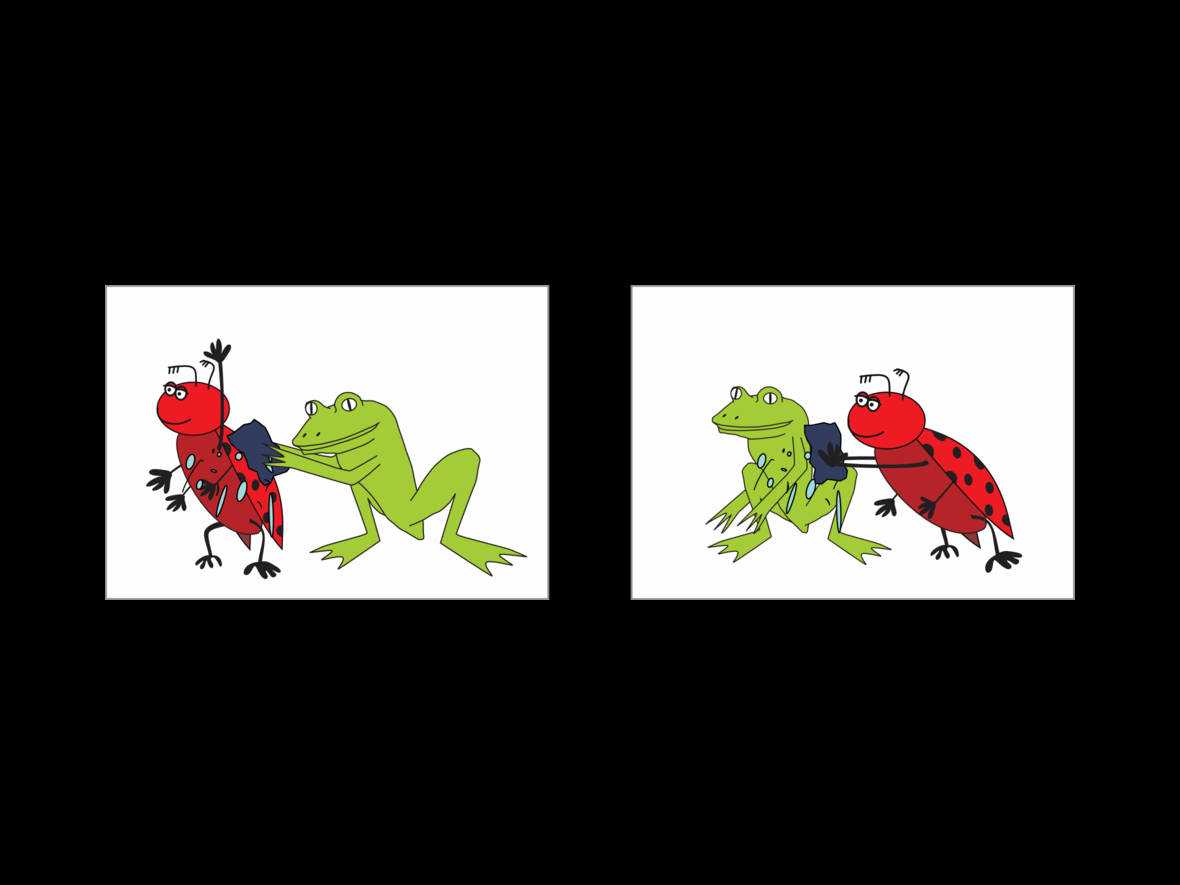
\includegraphics[width=0.75\textwidth]{pics/2_screen}
\caption{\label{2.screen} Example of a typical visual stimulus before the response}
\end{center}
\end{figure}

The spoken sentences were always posed as questions in order to elicit an immediate response.
Each question was posed in a right-branching structure (see table \ref{2.sentences} for an example).
Object-relative clauses and subject-relative clauses were presented in random order at a ratio of 2.5:1.
Questions were voiced in a natural, child-directed tone by a professional native speaker.
The question consisted of an actor, a recipient and the verb that described their interaction.
The performed action was either painting, pushing, combing, washing, pulling or catching.
The actor and recipient were selected randomly from 12 different races: Lion, rabbit, wolf, bird, fox, hedgehog, dog, tiger, ape, ladybug, bear and frog.
No two identical races appeared in the same picture.

\vspace{5mm}
\begin{table}[htb]
\begin{center}
\begin{tabular}{c|cccccccc}
Original & Wo & ist & der & K"afer, & den & der & Frosch & w"ascht?\\
Translated & Where & is & the & bug$_{OBJ}$, & who$_{ACC}$ & the & frog$_{SUBJ}$ & washes?\\
Word index & 1 & 2 & 3 & 4 & 5 & 6 & 7 & 8
\end{tabular}
\caption{\label{2.sentences} Example stimulus sentence. Top: original spelling in German. Middle: Literal translation in English. Bottom: Word index within the sentence}
\end{center}
\end{table}
\vspace{5mm}

Immediately after each response, an icon appeared below the two animal pairs.
A green checkmark, a diagonal red cross and a yellow skip symbol signified a correct response, an incorrect response and an invalid trial, respectively.
The trial feedback screen was presented for a random interval between 400ms and 800ms.

This experiment created a tradeoff between speed and accuracy.
To encourage a high level of attention and a high number of usable trials, a feedback screen was displayed at the end of each cluster.
On this screen, two bar graphs visualized response speed and accuracy during the preceding cluster.

Visual and auditory stimuli were produced by a computer running the software package Presentation (Neurobehavioral Systems, Inc., version [14.6]).
Video signal was displayed by a 17-inch TFT display at a distance of approximately 80cm.
Sound was played with a pair of semi-open headphones.


\paragraph{Analysis}

Behavioral data were analyzed with Matlab (version 2014a).
Response accuracy was evaluated for the case that subjects responded randomly.
For this purpose, accuracy was compared to the outcome of a random sequence of binary events.
We established the alpha = 0.01 confidence interval for the percentage of correct trials ($\frac{k}{n}$) that could be answered correctly purely by chance.
This calculation was implemented using the binomial fit method in Matlab: binofit(k, n, alpha).
If the upper confidence interval of this calculation exceeded the subject-specific accuracy, the subject was removed from further analysis.
Two subjects failed to exceed chance level performance, leaving 19 subjects for the analysis.

Two types of behavioral data were analyzed for group and condition effects: response time (RT) and response accuracy (RA).
Response time was measured at the condition onset, i.e. at the "'d"' sound of the sixth word.
Trials were omitted when the subject skipped or answered them incorrectly, or responded earlier than the cue.
Accuracy was calculated by dividing the amount of correct trials by the amount of total trials for each subject.

A Shapiro-Wilk test was used to test for normal-distributed residuals.
Accuracy passed this test at a p = 0.01 significance level.
The impact of the syntactic condition on response accuracy was determined with a T-test.

Any unintended bias on response time was determined by splitting RT from each subject into two groups along one of five impact factors.
The two groups were then compared with a T-test.
The five grouping factors were response side (left / right), condition (object-relative / subject-relative), the race of the actor (12) and recipient (12) and the peformed action.

\paragraph{Results}

Subjects responded after a median delay of 2.0s (quickest 5\%: 1.0s, slowest 5\%: 5.2s).
The median accuracy was 70\% (worst 5\%: 62\%, best 5\%: 94\%).
The syntactic condition had a highly significant effect on accuracy (p < 0.001, t(18) = -14.0).
No factor had a significant effect on response time (p > 0.1, F < 1.5).

\begin{figure}[h]
\begin{center}
\vspace{7mm}
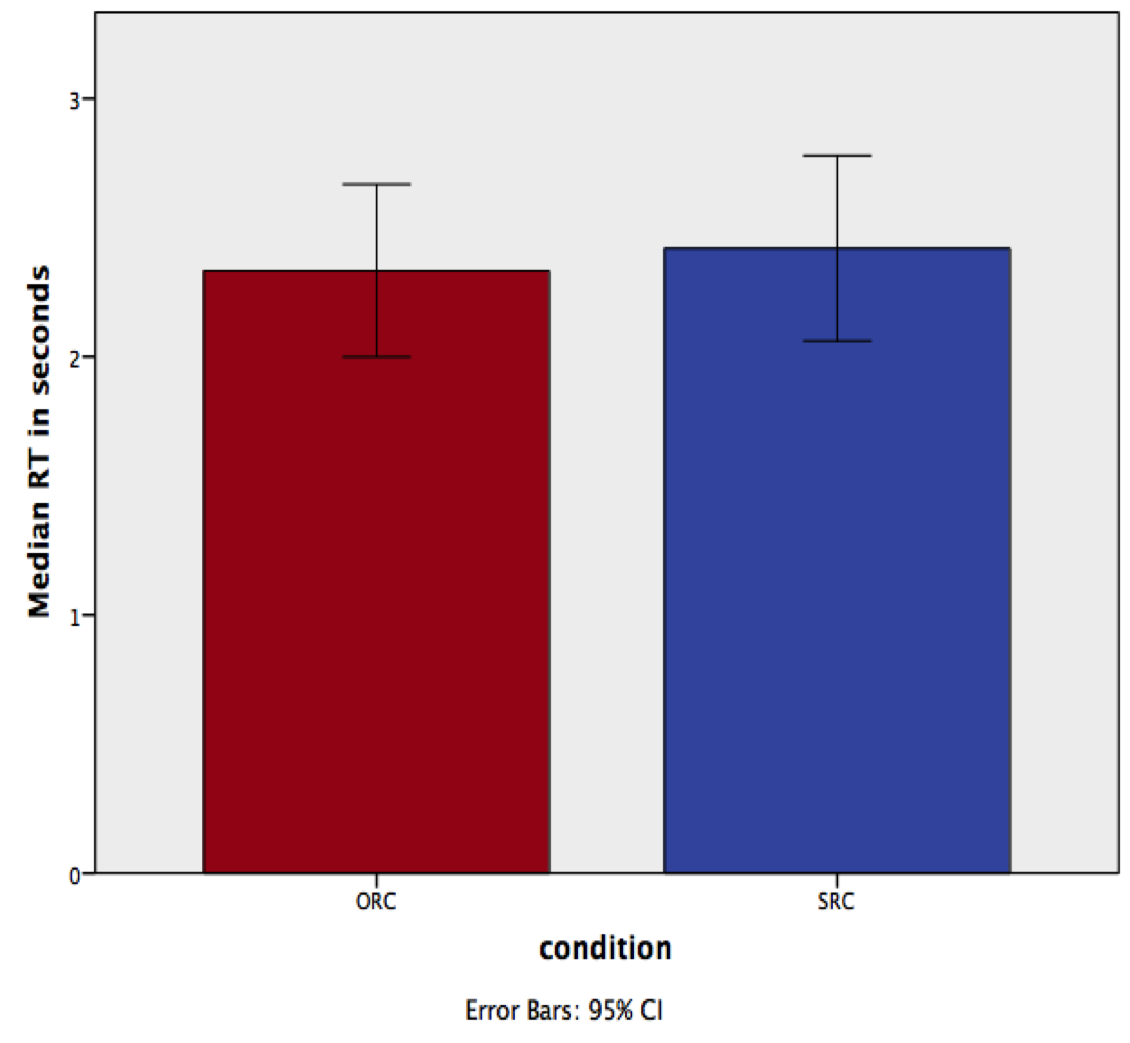
\includegraphics[width=0.45\textwidth]{pics/2_RTgraph}
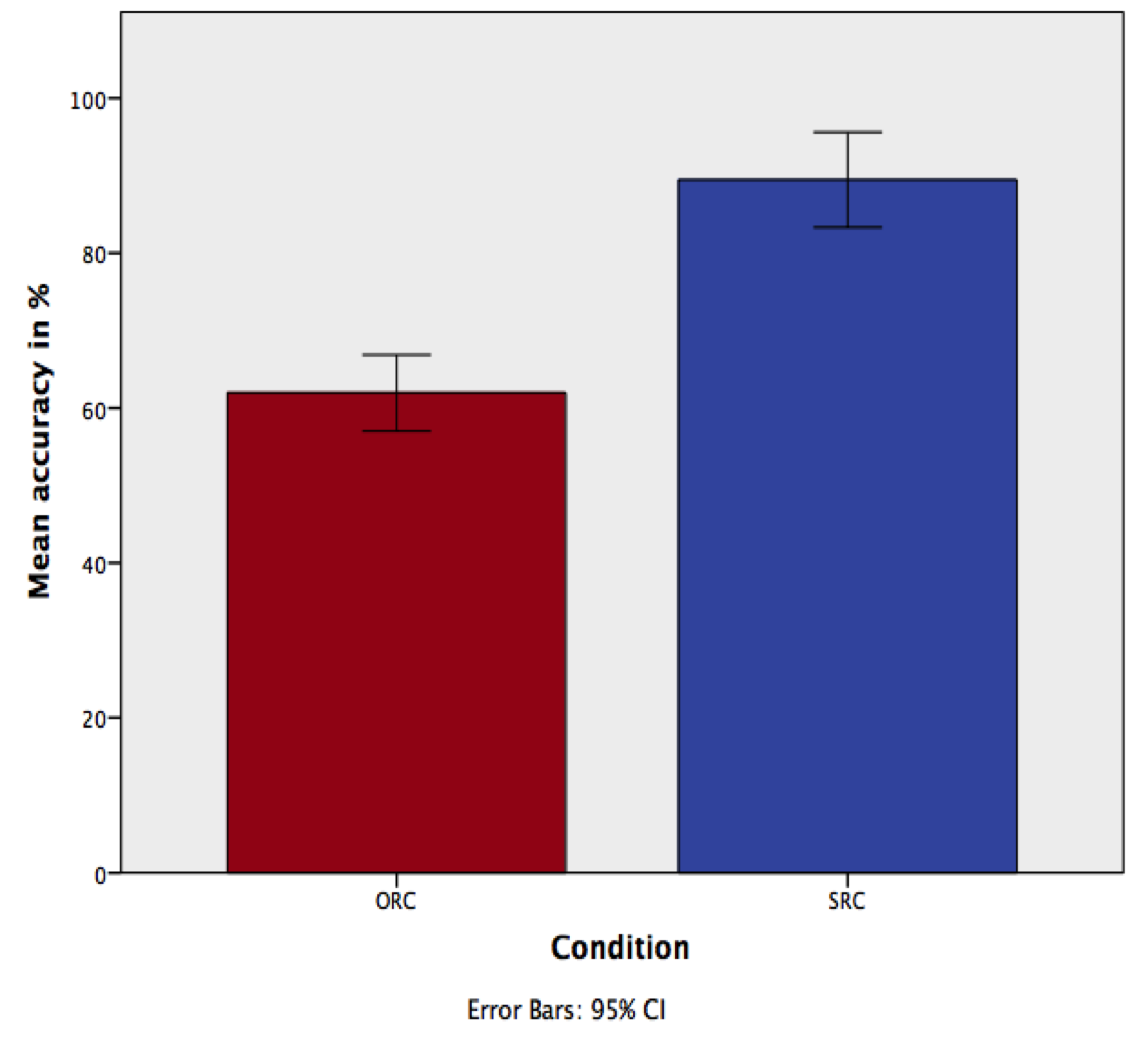
\includegraphics[width=0.45\textwidth]{pics/2_RAgraph}
\caption{\label{2.RTgraph} Chart of the grand average performances for subject-relative (blue) and object-relative (red) clauses. Left: Median response time from conditional onset. Right: Average response accuracy.}
\end{center}
\end{figure}

Post-hoc tests were conducted to reveal condition-specific accuracy values.
The average accuracy for responses to subject-relative clauses was much higher than to object-relative clauses (93\% and 64\%, respectively).
Due to the proximity to a 50\% chance level, we repeated the binomial fit test of individual accuracy, exclusively with responses to object-relative clauses.
8 of 19 subjects failed this test at a p = 0.01 significance level.
After removing these subjects from the analysis, selected tests were repeated.

Median response times remained unchanged for both conditions.
Overall accuracy in the remaining subjects improved slightly (95\% for subject-relative clauses and 68\% for object-relative clauses).
The difference in accuracy between conditions weakened slightly (p < 0.001, t(10) = -9.4).


\paragraph{Discussion}

The first goal of this pilot study was to establish an unbiased test paradigm.
The variation in grammatical elements had no undesired impact on response times.
Syntax conditions produced a strong effect in both performance metrics.
These findings support the current stimulus setup for use during MEG measurements.


The second goal of the pilot study was to determine if 10-year old children were suitable subjects for the designed task.
Accuracy levels were comparable with the findings of similar experiments.
Due to different trigger points and sentence lengths, comparisons of response times couldn't be made directly and were instead limited to comparisons of effect size.
We start by comparing our results to our spiritual predecessor, the study by [2.1].
They found no significant conditional impact on response time in the 9-10-year age bracket.
In stark contrast to our results (93\% and 64\% for subject- and object-relative clauses), their subjects were not influenced by a condition effect, with accuracy levels of 94\% in both conditions.
The good performance was met with surprise and speculation that semantic cues may have helped with sentence comprehension.
This speculation was supported by their fMRI findings, which indicated that children relied heavily on semantic-centric processing areas, rather than on pure syntax-related processing areas that adults use.
Our setup didn't include semantic cues, which puts our results more in line with other infant studies.

[2.2], for instance, measured repetition performance in 3- and 4-year-old children.
The study presented German subject-relative and object-relative clauses with two interacting people in third person, similar to our setup.
Their subjects performed with an accuracy of just 5\% (3 years) and 26\% (4 years) for object-relative clauses.
Subject-relative clauses were performed with 13\% and 31\% accuracy, respectably.
Note that these ratings represent accurate verbal repetition, and don't need to be corrected for chance level performance.

[2.3] found more accurate responses to portuguese right-branching subject- and object-relative clauses.
Subject-relative clauses were correctly answered 23\%, 50\%, 83\% and 80\% of the time (in 3-, 4-, 5- and 6-year old children, respectably).
Object-relative clauses reached only slightly lower accuracy levels of 18\%, 40\%, 75\% and 68\%, respectably.
They employed a more user-friendly approach by requiring the children to act out the posed sentences with toy animals.
Because the authors deliberately removed as many processing constraints as possible, these accuracy levels can be considered upper performance limits on these age brackets.

6 to 8 year old children solved syntactic problems with higher complexity in the study by [2.4].
The experimental design varied two syntactical factors and one contextual factor.
One syntactical factor, "'question"', varied English object- and subject-relative clauses, coinciding with our setup.
Object-first and subject-first clauses were responded with an accuracy of 64\% and 83\%, respectably.

Response time and accuracy performance indicates that the 10-year age bracket was successful in selecting subjects with an incomplete dorsal tract II.
Compared to typical adults, our subjects performed considerably worse in both accuracy and response time.
Compared to younger children, our subjects performed condsiderably better in subject-relative clauses.

42\% of our subjects failed to perform better than chance level when the task required a fully-developed AF.
We have no sufficient reason to assume that these subjects were using a random-button strategy.
If anything, the weakened condition effect indicates that these performances were due to honest mistakes.
Hence, there is no reason to exclude subjects with chance-level performances to object-relative clauses.


Finally, the pilot study revealed a few design flaws as well.

First, sentences differed systematically between conditions even before the intended condition cue.
The syntactical condition reverses the order of pronouns, creating an opposition between "'der den"' and "'den der"'.
To prevent confounding effects from different content, the initial sentence fragment needs to be identical at least across conditions, and, preferably, across trials as well.
Ideally, the distance between the end of this identical sentence fragment and the conditional cue point should be as short and invariant as possible.

Second, our sentence structure contained a theoretical loophole.
With sufficient time and wit, subjects could develop an alternative strategy that doesn't require syntactic processing of the whole sentence.
The alternative strategy exploits the fact that the minimum information for a correct decision is already available at the fifth word (see table \ref{2.1.sentences}).
Subjects only needed to complete three sequential steps:
First, attending only to the left of the two pictures.
Second, waiting until the fourth word is spoken.
If the mentioned animal was displayed as actor, the left button would be correct and vice versa.
Third, using the fifth word to execute the previous or the reverse button mapping.
If the mentioned word was a "'der"', the previously correct button remained correct and could be pressed immediately.
If the mentioned word was a "'den"', the previously wrong button had to be pressed for a correct result.
This strategy could potentially reduce the task into a simple series of motor preparation and pattern matching.
Complex syntactic processing and, presumably, the use of pSTS and dorsal pathway II would be circumvented.
Employing this strategy could create suspicious behavioral results in the form of systematically reduced and less varied response times.
This flaw was the main reason for the redesign of stimuli for the main study.